% `template.tex', a bare-bones example employing the AIAA class.
%
% For a more advanced example that makes use of several third-party
% LaTeX packages, see `advanced_example.tex', but please read the
% Known Problems section of the users manual first.
%
% Typical processing for PostScript (PS) output:
%
%  latex template
%  latex template   (repeat as needed to resolve references)
%
%  xdvi template    (onscreen draft display)
%  dvips template   (postscript)
%  gv template.ps   (onscreen display)
%  lpr template.ps  (hardcopy)
%
% With the above, only Encapsulated PostScript (EPS) images can be used.
%
% Typical processing for Portable Document Format (PDF) output:
%
%  pdflatex template
%  pdflatex template      (repeat as needed to resolve references)
%
%  acroread template.pdf  (onscreen display)
%
% If you have EPS figures, you will need to use the epstopdf script
% to convert them to PDF because PDF is a limmited subset of EPS.
% pdflatex accepts a variety of other image formats such as JPG, TIF,
% PNG, and so forth -- check the documentation for your version.
%
% If you do *not* specify suffixes when using the graphicx package's
% \includegraphics command, latex and pdflatex will automatically select
% the appropriate figure format from those available.  This allows you
% to produce PS and PDF output from the same LaTeX source file.
%
% To generate a large format (e.g., 11"x17") PostScript copy for editing
% purposes, use
%
%  dvips -x 1467 -O -0.65in,0.85in -t tabloid template
%
% For further details and support, read the Users Manual, aiaa.pdf.


% Try to reduce the number of latex support calls from people who
% don't read the included documentation.
%
\typeout{}\typeout{If latex fails to find aiaa-tc, read the README file!}
%


\documentclass[]{aiaa-tc}% insert '[draft]' option to show overfull boxes
\usepackage{amssymb}
\usepackage{amsmath}
\usepackage{listings}
\usepackage{graphicx,xcolor}
\usepackage{svg}
\pagestyle{plain}
\usepackage{fancyhdr}
\usepackage{wasysym}
\usepackage{textcomp}
%\usepackage{lastpage}
% 
%\pagestyle{fancy}
%\fancyhf{}
% 
%\rfoot{Page \thepage \hspace{1pt} of \pageref{LastPage}}
%\setcounter{page}{1}
\pagenumbering{arabic}

\usepackage{color}
 
\definecolor{codegreen}{rgb}{0,0.6,0}
\definecolor{codegray}{rgb}{0.5,0.5,0.5}
\definecolor{codepurple}{rgb}{0.58,0,0.82}
\definecolor{backcolour}{rgb}{0.95,0.95,0.92}
 
\lstdefinestyle{mystyle}{
    %backgroundcolor=\color{backcolour},   
    commentstyle=\color{codegreen},
    keywordstyle=\color{blue},
    numberstyle=\tiny\color{codegray},
    stringstyle=\color{codepurple},
    basicstyle=\footnotesize,
    breakatwhitespace=false,         
    breaklines=true,                 
    captionpos=b,                    
    keepspaces=true,                 
    numbers=left,                    
    numbersep=5pt,                  
    showspaces=false,                
    showstringspaces=false,
    showtabs=false,                  
    tabsize=2
}
 
\lstset{style=mystyle}

 \title{Design Optimization for a Student-Built \\ Sub-Orbital Rocket}

 \author{
  Ondrej Fercak\\
  Erin S. Schmidt\\
  %\and
  Ian Zabel\\  
 }

 % Data used by 'handcarry' option if invoked
 %\AIAApapernumber{YEAR-NUMBER}
 %\AIAAconference{Conference Name, Date, and Location}
 %\AIAAcopyright{\AIAAcopyrightD{YEAR}}

 % Define commands to assure consistent treatment throughout document
 \newcommand{\eqnref}[1]{(\ref{#1})}
 \newcommand{\class}[1]{\texttt{#1}}
 \newcommand{\package}[1]{\texttt{#1}}
 \newcommand{\file}[1]{\texttt{#1}}
 \newcommand{\BibTeX}{\textsc{Bib}\TeX}

\begin{document}

\maketitle

\begin{abstract}
Students at Portland State University are working to build the first student-built rocket to fly above the 100 km von Karman line. To date there have been few examples of numerical convex design optimization applied to the problem of such experimental student-built rockets. A Runge-Kutta integration trajectory simulation was built with Python. This was used to perform a Simplex Search optimization with the goal of optimizing rocket GLOW. The optimization has identified a concept for a rocket with a 113 kg GLOW, design thrust of 3.2 kN thrust (sea-level), expansion ratio of 4.7, diameter of \diameter11" capable of reaching the von Karman line.
\end{abstract}

\section*{Nomenclature}

\begin{tabbing}
  XXX \= \kill% this line sets tab stop
  PSAS \qquad Portland State Aerospace Society\\
  $h$ \qquad Altitude (m)\\
  $\dot{m}$ \qquad  Mass flow rate (kg/s)\\
  $D$ \qquad Airframe diameter (in)\\
  $L$ \qquad Total propellant tank length (m)\\
  $TWR$ \qquad Thrust-to-Weight Ratio \\
  $p_e$ \qquad Nozzle exit pressure (kPa)\\
  $p_{ch}$ \qquad Combustion chamber stagnation pressure (kPa)\\
  $m$ \qquad Mass (instantaneous) (kg)\\
  $g$ \qquad Constraint vector\\
  $x$ \qquad Design vector\\
  GLOW \qquad Gross-Lift-Off-Weight (kg)\\

 \end{tabbing}

\section{Introduction}
There is an emerging demand by both governments and private industry for small 'venture class' launch vehicles to deliver nano-satellites into Low Earth Orbit (LEO). While there are yet few operational examples of such dedicated small satellite launch vehicles, they would likely share cladistic similarities, at the extrema of their size and mass envelope range, with both large orbital launch vehicles and the comparatively small high-powered rockets that have been operated by hundreds of amateur and university groups for decades. Typically high-powered rockets fly ballistic trajectories with apogees generally less than 10 km above sea-level. However, several amateur and university groups harbor aspirations of sub-orbital flight above the von Karman line 100 km above the surface of the Earth. As of the Spring of 2016 the current record holder for altitude at apogee by a student organization is TU Delft's Delft Aerospace Rocket Engineering (DARE) team which reached 21.457 km with their Stratos II+ rocket on October 16, 2015\cite{dare}.

The Portland State Aerospace Society (PSAS) is an engineering student organization and citizen science project located at Portland State University dedicated to developing low-cost, open-source, and open-hardware high-powered rockets and avionics systems with special interests in small launch vehicle technology and nanosatellites\cite{PSAS}. In 2015 PSAS initiated a project to build and fly it's own entry in this rapidly intensifying `university space race'.

Herein, we apply design optimization methodology to the problem of design and trajectory optimization of small sounding rockets, and particularly to the PSAS's LV4 `space rocket'. This rocket will leverage powerful liquid-fuel propulsion, an extremely light-weight carbon-composite airframe, full 6-DoF attitude control and active stabilization. LV4 is intended to fly with a design apogee of over 100 km, and is currently planned for launch by 2021. A SolidWorks CAD render of a concept for LV4 is shown in Figure \ref{fig:rocket}.

\begin{figure}[h!]
  \centering
  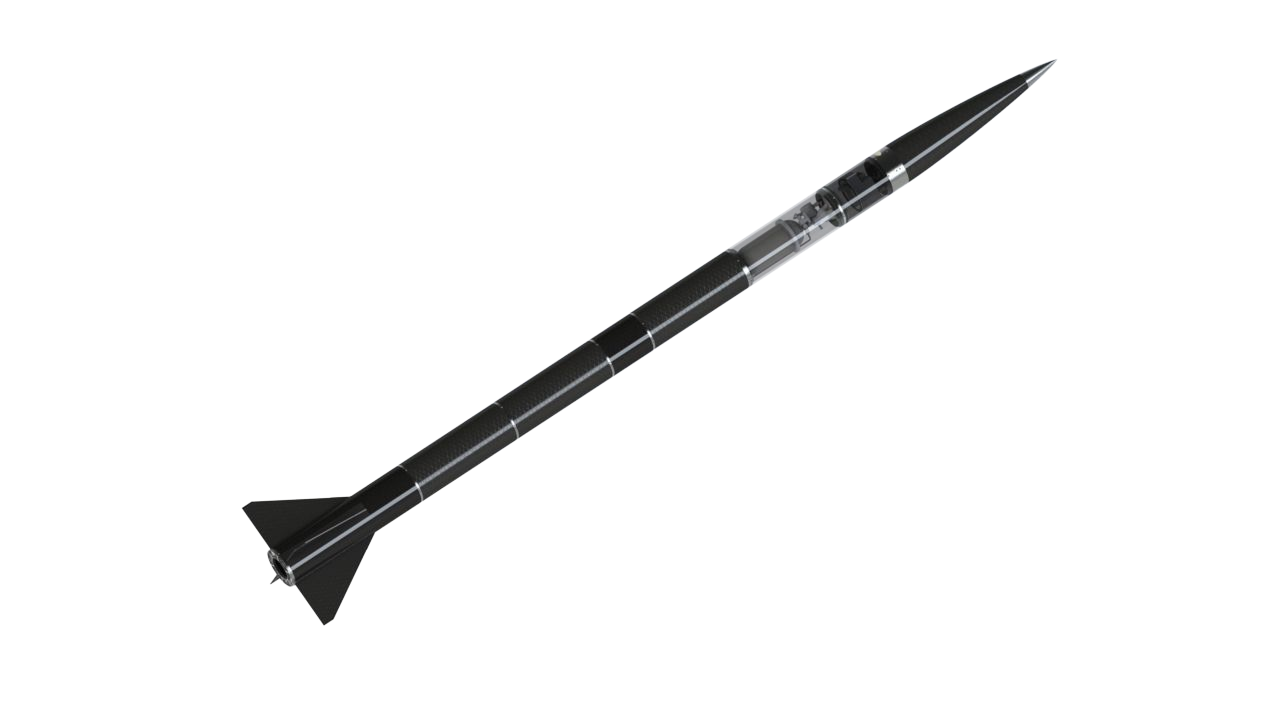
\includegraphics[width=0.9\linewidth]{Figures/LV4_render.png}
  \caption{SolidWorks CAD render of an early design phase concept of the PSAS LV4 sub-orbital rocket.}
  \label{fig:rocket}
\end{figure}

\section{Methods}
\subsection{Problem Definition}
Clean-sheet conceptual design and trajectory optimization of launch vehicles is a classically difficult problem. This problem arises for two reasons. The first is that the trajectory equation is a 2nd order non-linear ordinary differential equation with coefficients that are themselves described by non-linear first and second order ODE's. This problem has no closed-form solution. Secondly, detailed design choices in propulsion, structures/weights, aerodynamics, and guidance and control which ultimately all appear as variables in the governing equation are both highly coupled and non-hierarchical. Schematically the coupling between the variables is presented in Figure \ref{fig:coupling}. The traditional approach to dealing with this problem has been to evaluate vehicle performance by examining the value of each parameter by fixing the values of the remaining parameters e.g. the ``one variable-at-a-time" trade-off analysis approach. However there are several important limitations to this approach:
\begin{itemize}
\item Conceptual design is usually carried out with low-fidelity models
\item Some relationships among the design variables are poorly understood
\item Optimizing individual design variables does not guarantee optimality at the overall system level
\end{itemize}

In practice this results in a highly iterative design process and concomitant requirement mismatches, developmental dead-ends and sub-optimal final design. The problem with sub-optimal design is magnified by the ramifications of Konstantin Tsiolkovsy's equation, with the severe implication of exponential growth in design requirements for linear increases in rocket dry mass. Since ultimately all design decisions impact the rocket dry mass in some way it is imperative to understand these trade-offs and compromises as early in the design process as possible to reduce the potential for technical, schedule, and cost risks. This is especially the case for time, technical expertise, and funding constrained student organizations. Therefore there is a strong motivation to treat the conceptual design parameters ``all-at-once" using applied optimization techniques. A numerical design optimization approach allows us o systematically explore a vast trade space under a realistic timeframe.

Some commercial and/or governmental tools exist for launch vehicle design optimization. These include codes such as FASTPASS \cite{Fastpass}, and SWORD\cite{SWORD}. There are also open-source design and optimization tools that can be applied to high-powered rocketry such as Open Rocket\cite{openrocket}, or JSBSim\cite{jsbsim}, however these tools either cannot be run in a batch mode or lack I/O tools to support direct numerical optimization. In the context of this developing interest in clean-sheet small launch vehicle designs we can identify a need for a design tool high-level enough for simplicity, speed, and ease of use, but which captures enough of the dimensions of the optimization problem to still be useful as a guide in the early conceptual design phase. This tool will use fairly low-fidelity models, and will be used for trajectory optimization, propulsion design, airframe sizing, and mass estimation. Per PSAS’s open-source mandate all (non-ITAR) project development deliverables are being made publicly available under a GNU GPL v2 license\cite{Git}. This code was written in Python because it is free and open-source, and for its inherent object-oriented modularity, numerical efficiency, and wide use in the community of scientific computing. It is hoped by the authors, and the members of PSAS, that the discourse around educational launch vehicles and their design will be elevated by making the information for this project publicly available.

\begin{figure}[ht]
    \centering
    \includesvg[width=0.7\textwidth]{coupling}
    \caption{Coupling and dependencies between various launch vehicle design disciplines.}
	\label{fig:coupling}
\end{figure}

\subsection{Objectives and Constraints}
The objective of the optimization is to minimize the total system complexity and cost of the 100 km launch vehicle. While these objectives can be abstract as numerical values in the early conceptual design phase, we expect them to scale closely with the initial mass of the launch vehicle (including the mass of loaded propellants), which is usually defined by the Gross Lift-Off Weight (GLOW) figure of merit.  

Thus we wish to minimize GLOW subject to practical model linearity and structural constraints. In the most practically usefully sense the design variables include thrust, airframe diameter and propellant tank lengths. However for numerical simplicity thrust will be expanded into mass flow rate and expansion ratio design variables, and then back-solved within the simulation. There are also a large number of design constants present in the models, which include specific impulse and combustion chamber pressure, propellant mixture ratio, and others, but which for the sake of brevity will be largely ignored in the following discussion. The model currently include 6 inequality constraints:

\begin{itemize}
\item Apogee: 100 km
\item Thrust-to-Weight Ratio (TWR): Trade-off between gravity loss and aerodynamic stability
\item Length to Diameter Ratio(L/D): Trade-off between aerodynamic stability and mechanical (non-rigid body) resonance modes
\item Maximum acceleration: Set by the material limits of various launch vehicle subsystems
\item Diameter: Manufacturability (current process scale-able from \diameter6" to up to \diameter14") 
\item Nozzle over-expansion: Prevents the assumption made to help linearize thrust model from becoming invalid
\end{itemize}

Mathematically the problem can be stated as

\[ \mbox{min} \hspace{2 mm} m_{initial} = m_{dry}(h) + m_{propellants,  initial}(h) \]
\begin{eqnarray*} \mbox{where} \hspace{5 mm} \begin{split}x = \left\{ \begin{array}{ll}      & \dot{m}\\
          & D\\
          & L\\
          & p_e \end{array} \right. 
          \end{split} \hspace{2 mm} \mbox{subject to} \hspace{2 mm} \begin{split}
          g = \left\{ \begin{array}{ll}
          & 5 \leq L/D \leq 15\\
          & TWR \geq 2\\
          & \frac{p_e}{p_a} \geq 0.5\\
          & 6 \leq D \leq 14\\
          & h \geq 100000\\
          & \frac{a_{max}}{g_0} \leq 15 \end{array} \right. \end{split}\end{eqnarray*}

While the objective function itself is given by a very simple function of the design variables $D$ and $L$, the constraints require a much more complex model. The following section discusses the trajectory simulation model required to capture values of these constraints for any particular design vector.

\subsection{Trajectory Simulation}
The trajectory of the rocket, in a single degree of freedom, can be best described by altitude $h(t)$, velocity $V(t)$, and total mass $m(t)$ state variables which are functions of time. The initial values of the state variables are given by $h_0$, $V_0$, and $m_0$ respectively. The governing equation of the rocket trajectory is Newton's 2nd law of motion 

$$F = \frac{d(mV)}{dt}.$$

This can be expanded in terms of the sum of forces acting on the rocket during free flight going up to apogee

$$Thrust(h) - Drag\left(h, \frac{dh}{dt}, \left(\frac{dh}{dt} \right)^2 \right) - m\left(\frac{dm}{dt}, t\right)g_0 = \frac{d}{dt} \left(m \frac{dh}{dt}\right).$$

We usually express drag as
\[F_d = \frac{1}{2} \rho V^2 C_d A\]

where $\rho$ is the local air density, $A$ is the frontal area, $C_d$ is the drag coefficient which for a given airframe geometry is a function of angle-of-attack (which for a 1-DoF system is identically zero), and Mach number. The Mach number is a function given by

\[ \frac{V}{c} = \frac{V}{\sqrt{kRT}} \]

where $c$ is the local speed of sound, $k$ is the gas ratio of specific heats, $R$ is the specific gas constant, and $T$ is the gas temperature. These numbers are supplied, as well as $\rho$, and $p_a$ the ambient pressure, are supplied by the 1976 U.S. Standard Atmosphere model. For simplicity, drag coefficients are interpolated from published aerodynamic data from the 1950's era NACA/USN/NASA Aerobee-150 sounding rocket class, which is expected to be dimensionally similar to the LV4 sounding rocket\cite{aerobee}.

The rocket thrust force, given a huge number of simplifying assumptions, is a function of the mass flow rate design variable, the chamber pressure constant, and the ambient pressure state variable. It is given by
\[F_t = \dot{m}V_e + A_e(p_e - p_a) \]

where $V_e$ is the rocket exhaust velocity, $A_e$ is the rocket nozzle exit area. The exhaust velocity, again given a large number of simplifying assumptions, is given by

\[V_e = \sqrt{\frac{2kRT_{ch}}{k - 1}\left(1 - \left(\frac{p_e}{p_{ch}}\right)^{((k - 1)/k)}\right)}\]

where $T_{ch}$ is the chamber pressure, which along with the combustion chamber gas ratio of specific heats $k$, and gas constant $R$ are functions of the mixture ratio of the propellants, and the chamber pressure $p_{ch}$ determined using the NASA Chemical Equilibrium Analysis (CEA)\cite{CEA} tool and are design constants. It should be noted that the $p_e$ is a design variable tied to the expansion ratio of the rocket engine, but that $p_a$ is constantly changing with altitude. The thrust function is maximized when $p_e = p_a$, however this occurs at one, and only one, altitude. Thus the design expansion ratio selection directly benefits from trajectory optimization.

By finite-differencing the derivatives of the governing equation a zeroth-order Runge-Kutta integration (e.g. Forward Euler) of the governing equation is used to determine the rocket trajectory. This approach was chosen only for simplicity; in principle central differencing or trapezoidal integration are more generally accurate discretization approaches. Forward Euler difference equations always have the form

\[y_{i+1} = y_i + \left(y\hspace{-1 mm}-\hspace{-1 mm}\mbox{rate at } t_i \right)(t_{i+1} - t_i) \]

where $y(t)$ is the state variable being integrated, and $i$ is the time index superscript. In this way the state variables $h$, $V$, and $m$ can be defined at any discrete time $t_0$, $t_1$, $t_2$ ... $t_i$. Given a vector of the four design variables the trajectory function returns numerical values of the objective function and constraint vector. This trajectory code was benchmarked against known trajectory and design date for both the Aerobee-150 and Armadillo Stig-B sounding rockets, and the results compare favorably. This grants us at least some confidence in the assumptions made in the model. The Python trajectory module code can be found in the appendices.

\subsection{Optimization Approach}
There are several general approaches to design optimization for launch vehicle design found in literature:
\begin{enumerate}
\item Design of Experiments methods (Taguchi Methods\cite{Taguchi} \hspace{0.1 mm}, Response Surface Methods\cite{RSM})
\item Gradient methods (steepest descent)
\item Stochastic methods (genetic algorithm\cite{genetic}, simulated annealing)
\end{enumerate}
While there are certain advantages to each of these approaches, only gradient based methods were within the scope of the ME596 class. Furthermore the difficulty of differentiating the governing equations, the expected multi-modal nature of the response surface and the discrete nature of some of the variables ($m$, $C_d$, etc.) argue against gradient based methods. We therefore selected a gradient free, non-stochastic approach: the Nelder-Mead method (e.g. Simplex Search). The limitations of this choice may become evident for high-dimension problems, but for $x \in \textbf{R}^4$, we expect the algorithm have major problems with convergence. Inequality constraints were handled by using an exterior penalty function. The pseudo-objective function as finally implemented is given by
\begin{verbatim}
obj_func = m[0] + rp*(max(0, (L+2)/(dia*0.0254) - 15)**2 + max(0, -TWR + 2)**2 \
+ max(0, -S_crit + 0.35)**2 + max(0, -alt[-1] + 100000)**2 + max(0, max(abs(a))/9.81 - 15)**2)
\end{verbatim}

The principle difficulties involved in the implementation of this algorithm (beyond those faced in earlier ME596 homework) were generalizing the algorithm reflection case handling, and initial simplex vertices generation to $\textbf{R}^4$ space. The Python Simplex Search module code can be found in the appendices.

\subsubsection{Qualitative Discussion of Algorithm Behavior}
While the optimization algorithm has proven to be excellent at quickly finding feasible design given any initial guess of the design variables $x_0$, it has also exhibited issues with convergence, and parameter sensitivity. This is often manifested by next-step iterative reflection points becoming trapped in a loop. In practice this causes the current best design point to move closer to an optimum in large "fits and spurts". Another problem is that there appear to be many optima points with similar pseudo-objective function values, but different design points. This leads to a large sensitivity to $x_0$, $\alpha$, $\gamma$ and $\beta$ parameter choices. Some attempt was made to  smooth out the performance of the algorithm by non-dimensionalizing all of the function values in the pseudo-objective function. This helps prevent numerically large constraints from prejudicing over much the final optimum, and makes the choice of $r_p$ seem hopefully less arbitrary. 

\subsubsection{Benchmarking}
To ensure that the code written is providing accurate and sensible results, the output and code was benchmarked against test cases with simple analytical solutions and against an off-the-shelf Nelder-Mead algorithm. 

One method of confirming the results is to apply a provided homework problem and respective solution, and check to see if the output correlates with the known answer. Since a previous homework problem for ME 596 required a simplex search, that problem was applied to the code written for the final project. The results correlated with an answer determined using classical analytical methods. The full launch vehicle design optimization problem results were also benchmarked against the SciPy \cite{scipy} Python optimization library. The \begin{verbatim}scipy.optimize.minimize(f, x_0, method='nelder-mead') \end{verbatim} results often offered slight improvements in optimized GLOW compared with those from our own code for a given $x_0$. The SciPy minimize function also ran much faster than our own, at least 2 orders of magnitude less physical time for the same number of iterations.

\section{Results}
The results of the design optimization in terms of the optimization design variables and a number of derived secondary design variables are presented in Table \ref{table:outputs}. Various state variables for the trajectory of the optimized LV4 design are plotted against time in Figure \ref{fig:trajectory}.

\begin{table}
\centering
	\begin{tabular}{l|l}
		\hline
		$\textbf{Parameter}$&$\textbf{Output}$\\
		\hline
		Optimized Design Vector & [1.2, 1.4, 10.8, 68.2]\\
		Initial Guess & [1.0, 1.6, 12.0, 50.0]\\
		Tankage Length & 1.2 m\\
		Mass Flow Rate & 1.4 kg/s\\
		Airframe Diameter & 10.8 in.\\
		Nozzle Exit Pressure & 68.2 kPa\\
		Iterations & 279\\
		Design GLOW & 112.8 kg\\
		Initial GLOW & 114.7 kg\\ \\
		\hline
		$\textbf{Constraints}$&\\
		\hline
		L/D ratio ($\leq15$) & 11.7\\
		Sommerfield Criterion ($\geq0.3$) & 0.7\\
		Max Acceleration ($\leq15$) & 6.7 g's\\
		TWR at Liftoff ($\geq2$) & 1.9\\
		Apogee Altitude & 100 km\\ \\
		\hline
		$\textbf{Additional Information}$&\\
		\hline
		Mission Time at Apogee & 176 s\\
		Total Propellant Mass & 70 kg\\
		Thrust (sea level) & 3.2 kN\\
		Thrust (vacuum) & 3.6 kN\\
		Burn Time & 53 s\\
		Expansion Ratio & 4.7\\
		Throat Area & 1.5 $\mbox{in.}^2$\\
		isp & 245 s\\
		Chamber Pressure & 350 psi\\
		Delta-V & 2.4 km/s\\
		Required Delta-V & 1.4 km/s\\	
	\end{tabular}
\caption{Optimized design parameters for the LV4 sub-orbital rocket.}
\label{table:outputs}
\end{table}

\begin{figure}[h!]
  \centering
  \includesvg{trajectory}
  \caption{Simulated trajectory up to apogee for an optimized LV4 design.}
  \label{fig:trajectory}
\end{figure}

It can be seen from the optimization results, an immediate take away is that a 100km sounding rocket can be constructed with a GLOW similar to that of liquid fueled rockets with apogees of less than 10 km. This feat is accomplished by the incredible mass savings of the inline monocoque  carbon-composite propellant tanks, as they drive down dry mass significantly compared with traditional welded aluminum tanks. This is a ramification of the exponential nature of Tsiolkovsky's problem, which can be seen in Figure \ref{fig:glowvsmdry} which shows the dependence of optimal GLOW on initial mass. Such tanks would only need to be 1.2 m long and roughly \diameter11". This is achievable with current manufacturing techniques developed by PSAS as part of a senior design project in 2014. Furthermore, the optimize design thrust required is only 3.6 kN in a vacuum. Such a rocket engine would only be marginally larger than the 2 kN engine already under development by PSAS as part of a 2016 senior design project. 

\begin{figure}[h!]
  \centering
  \includesvg[width=0.5\textwidth]{glow}
  \caption{Dependence of optimized GLOW on $m_{dry}$.}
  \label{fig:glowvsmdry}
\end{figure}

\section{Future Work}
There are many possible improvements to be made to the model, however we should still strive for a model with simple and straightforward inputs, and reasonable computation time. Some possible ways forward are outline below.

\subsection{Trajectory Model Improvements}
As stated previously the model presently uses the somewhat unphysical approach of determining drag coefficients by interpolating from a lookup table of historical data. However the data is based on a rocket with geometry that will undoubtedly be different from LV4. This is potentially a large source of error. There are 2 approaches to improving the $C_d$ calculation: by using an iterative approach where optimum values of length and diameter are determined from the optimizer, these are used with static stability analysis to design and size fins, mesh the CAD drawing of the concept and perform a compressible-flow CFD simulation (perhaps using CD-adapco Star CCM+) sweeping though Mach numbers. The improved $C_d$ tables would then be used in the next iteration of the optimizer. This process would be iterated until the GLOW converges. A second approach would be to calculate approximate $C_d$ values in a less accurate, but also much less manual labor intensive manner. This could be accomplished by calculating component-wise $C_d$ using Barrowman's method\cite{barrowman}. This would require adding a rotational degree of freedom to the trajectory simulation, as well as adding stability derivative constraints to the pseudo-objective function. This would also entail direct optimization of the design variables of the aerodynamic fins (including sweep line, root chord, tip chord, and panel span). If we include practical design problems such as fin flutter this could could possibly vastly increase the complexity of the problem. Additionally, Nelder-Mead may have difficulty with convergence with this number of design variables. Finally $g_0$ is presently assumed constant, and while this often seems a safe assumption in everyday experience, in actually it is a function of altitude. Thus the trajectory simulation fidelity could be improved by the addition of a gravity/geoditics model. The WGS84 model harmonic expansion of the gravitational field potential seems promising for this application. 

\subsection{Feed System Improvements}
Presently the feed system mass is simply a given a (very) approximate estimated mass value, and is not subject to optimization. However , in practice, the feed system mass should scale with the propulsion system thrust and chamber pressure. While there are numerous papers detailing mass and envelope estimation of feed system for large rocket engines, unfortunately there seems little published data for engines smaller than 50 kN. Given the strong impact of total dry mass on optimized GLOW this factor is potentially a large source of error.

\subsection{Structural Model Improvements}
Besides the fact that the carbon-composite airframe will double as the fuel tank liner in certain sections, the overall strength of the structure is of great consideration. The greatest structural loading will occur at the point of highest dynamic pressure, occurs just after Mach 1 according to the simulation in Figure \ref{fig:trajectory}. To determine the loadings at this point, CFD or a simplified analytical model is required. The aerodynamic shear, pressure, wind buffeting, and acceleration are all considerations that lead to determining the combined stresses on the airframe at this point. In the optimization code, the structural loading is limited by constraining acceleration to below 15 g’s. This must be expanded on to include constraints on the maximum velocity of the rocket to ensure the maximum dynamic pressure and structural stresses are not too high. Some post-hoc FEA analysis is also justified to determine that the carbon-composite propellant tanks will not fail with the planar density assumed in the trajectory dry mass model.

\section{Conclusion}
Clean-sheet design of small launch vehicles, of both the orbital and suborbital varieties, is an area of rapidly increasing interest. However there is little published work regarding optimization of such vehicles in the early conceptual design phase. However identifying feasible designs and relationships between different design variables early in the design process is crucial to mitigating cost and schedule risks. Given this motivation a simple and fast, high-level code for design optimization of university group scaled sub-orbital rockets was developed using Python. The code benchmarks well compared with historical rocket designs and highlights exciting paths forward in terms of technology development for such vehicles. Given PSAS's interested in building the first university rocket to fly about the 100 km `threshold of space' this work will guide the groups technology development pathways, and inform requirements for future senior capstone projects sponsored by the organization for years to come.

\begin{thebibliography}{9}% maximum number of references (for label width)
%cite ideas: a few similar MDO papers, envelope estimation, scipy, PSAS
\bibitem{dare}
{\it Delft Aerospace Rocket Engineering.} DARE. Accessed June 5, 2016. http://dare.tudelft.nl/\\

\bibitem{PSAS}
{\it Portland State Aerospace Society.} PSAS. Accessed February 25, 2016. http://psas.pdx.edu.\\

\bibitem{Fastpass}
Szedula, J.A., {\it FASTPASS: A Tool For Launch Vehicle Synthesis}, AIAA-96-4051-CP, 1996.\\

\bibitem{SWORD}
Hempel, P. R., Moeller C. P., and Stuntz L. M., {\it “Missile Design Optimization Experience And Developments”}, AIAA-94-4344,1994-CP.\\

\bibitem{openrocket}
{\it OpenRocket}, Accessed June 5, 2016. http://openrocket.sourceforge.net/documentation.html

\bibitem{jsbsim}
Berndt, Jon S., {\it JSBSim: An Open Source Flight Dynamics Model in C++}. AIAA Modeling and Simulation Technologies Conference and Exhibit. Aug. 2004.

\bibitem{Git}
{\it Portland State Aerospace Society.} GitHub. Accessed February 25, 2016. https://github.com/psas.\\

\bibitem{aerobee}
Pressly, E. C., et al. {\it Sounding rockets for transporting scientific instruments in nearly vertical trajectory}, NASA, United States 1965, (pg. 58).\\

\bibitem{CEA}
Gordon, Sanford, and Bonnie J. McBride, {\it Computer program for calculation of complex chemical equilibrium compositions and applications}. National Aeronautics and Space Administration, Office of Management, Scientific and Technical Information Program, 1996.

\bibitem{Taguchi}
Stanley, D. O., Unal, R., and Joyner, C. R., {\it "Application of Taguchi Methods to Dual Mixture Ratio Propulsion System Optimization for SSTO Vehicles"}, Journal of Spacecraft and Rockets, Vol. 29, No. 4, 1992, pp. 453-459.\\

\bibitem{RSM}
Stanley, D. O., Engelund. W. C., Lepsch. R. A., McMillin, M. L.Wt K. E.. Powell. R. W., Guinta. A. A., and Unal, R., {\it "Rocket-Powered Single Stage Vehicle Configuration Selection and Design"}, Journal of Spacecraft and Rockets,Vol. 31, No. 5, 1994. pp. 792-798; also AIAA Paper93-Feb. 1993.\\

\bibitem{genetic}
Anderson, M., Burkhalter J., and Jenkins R., {\it “Multidisciplinary Intelligence Systems Approach To Solid Rocket Motor Design, Part I: Single And Dual Goal Optimization"}. AIAA 2001-3599, July, 2001.\\

\bibitem{scipy}
Eric Jones and Travis Oliphant and Pearu Peterson and others, {\it SciPy: Open source scientific tools for Python}, 2001, Accessed June 5, 2016. http://www.scipy.org/.\\

\bibitem{barrowman}
Barrowman, James S. {\it "The practical calculation of the aerodynamic characteristics of slender finned vehicles."} NASA, United States, 1967.

\end{thebibliography}

\newpage
\pagestyle{empty}
\section*{Appendix}
Note that these codes can also be found on Github at\\ https://github.com/psas/liquid-engine-analysis/tree/master/optimization.
\subsection{Trajectory Simulation Python Script}
\begin{lstlisting}[language=Python]
from math import sqrt, pi, exp, log, cos
import numpy as np
import csv

# A simple forward Euler integration for rocket trajectories
def dry_mass(L, dia):
    m_avionics = 3.3                       # Avionics mass        [kg]
    m_recovery = 4                         # Recovery system mass [kg]
    m_payload = 2                          # Payload mass         [kg]
    m_tankage = 20.88683068354522*L*dia*pi # Tank mass Estimation [kg]
    m_engine = 2                           # Engine mass          [kg]
    m_feedsys = 20                         # Feed system mass     [kg]
    m_airframe  = 6                        # Airframe mass        [kg]
    return (m_avionics + m_recovery + m_payload + m_tankage 
    + m_engine + m_feedsys + m_airframe)   # Dry mass             [kg]

def propellant_mass(A, L, OF=1.3):
    rho_alc = 852.3             # Density, ethanol fuel [kg/m^3]
    rho_lox = 1141.0            # Density, lox          [kg/m^3]
    L_lox = L/(rho_lox/(rho_alc*OF) + 1)
    m_lox = rho_lox*L_lox*A     # Oxidizer mass         [kg]
    m_alc = rho_alc*(L-L_lox)*A # Fuel mass             [kg]
    return m_alc + m_lox        # Propellant Mass       [kg]

def std_at(h):                  # U.S. 1976 Standard Atmosphere
    if h < 11000:
        T = 15.04 - 0.00649*h
        p = 101.29*((T + 273.1)/288.08)**5.256

    elif 11000 <= h and h <25000:
        T = -56.46
        p = 22.65*exp(1.73 - 0.000157*h)

    else:
        T = -131.21 + 0.00299*h
        p = 2.488 * ((T + 273.1)/216.6)**(-11.388)

    rho = p/(0.2869*(T + 273.1)) # Ambient air density [kg/m^3]
    p_a = p*1000                 # Ambient air pressure [Pa]
    T_a = T + 273.1              # Ambient air temperature [K]
    return p_a, rho, T_a

def thrust(x, p_ch, T_ch, p_e, ke, Re, mdot):
    p_a = std_at(x)[0]                          # Ambient air pressure [Pa]
    p_t = p_ch*(1 + (ke - 1)/2)**(-ke/(ke - 1)) # Throat pressure      [Pa]
    T_t = T_ch*(1/(1 + (ke - 1)/2))             # Throat temperature   [K]
    A_t = (mdot / p_t)*sqrt(Re*T_t/ke)          # Throat area          [m^2]
    A_e = A_t*(2/(ke + 1))**(1/(ke - 1))*(p_ch/p_e)**(1/ke) * 1/sqrt((ke + 1)/(ke - 1)*(1 - (p_e/p_ch)**((ke - 1)/ke))) # Exit area [m^2]
    ex = A_e/A_t              # Expansion ratio
    alpha_t = [14, 11, 10, 9] # Lookup table of divergence angles, assuming 80% bell length
    ex_t = [5, 10, 15, 20]    # Lookup table of expansion ratios from alpha_t
    alpha= np.interp(ex, ex_t, alpha_t)
    lam = 0.5*(1 + cos(alpha *pi/180)) # Thrust cosine loss correction, even in extreme cases this is definitely not an O(1) effect 
    Ve = lam*sqrt(2*ke/(ke - 1)*Re*T_ch*(1 - (p_e/p_ch)**((ke - 1)/ke))) # Exhaust velocity                                  [m/s]
    F = mdot*Ve + (p_e - p_a)*A_e                                        # Thrust force, ignoring that isp increases w/ p_ch [N]
    return F, A_t, A_e, Ve

def drag(x, v, A, Ma, C_d_t, Ma_t):
    # Check Knudsen number and switch drag models (e.g. rarified gas dyn vs. quadratic drag)
    (p_a, rho, T_a) = std_at(x)
    
    #C_d_t = [0.15, 0.15, 0.3, 0.45, 0.25, 0.2, 0.175, .15, .15] # V2 rocket drag coefficient lookup table
    #Ma_t = [0, 0.6, 1.0, 1.1, 2, 3, 4, 5, 5.6]                  # V2 rocket Mach number lookup table
    C_d = np.interp(Ma, Ma_t, C_d_t)                            # Drag coefficient function
    q = 0.5 * rho * v**2                                        # Dyanmic pressure [Pa]
    D = q * C_d * A                                             # Drag force       [N]
    return D, q

def trajectory(L, mdot, dia, p_e, p_ch=350, T_ch=3500, ke=1.3, Re=349, x_init=0):
    # Note combustion gas properties ke, Re, T_ch, etc, determined from CEA
    # Physical constants
    g_0 = 9.81 # Gravitational acceleration [m/s^2]
    dt = 1     # Time step                  [s]
    ka = 1.4   # Ratio of specific heats, air  
    Ra = 287.1 # Avg. specific gas constant (dry air)
    
    # LV4 design variables
    dia = dia*0.0254       # Convert in. to m
    A = pi*(dia/2)**2      # Airframe frontal area projected onto a circle of diameter variable dia
    m_dry = dry_mass(L, A) # Dry mass, call from function dry_mass()
    mdot = mdot            # Mass flow rate [kg/s]
    p_ch = p_ch*6894.76    # Chamber pressure, convert psi to Pa
    p_e = p_e*1000         # Exit pressure, convert kPa to Pa

    # Initial conditions
    x = [x_init]
    v = [0]
    a = [0]
    t = [0]
    rho = [std_at(x[-1])[1]]
    p_a = [std_at(x[-1])[0]]
    T_a = [std_at(x[-1])[2]]
    m_prop = [propellant_mass(A, L)]
    m = [m_dry + m_prop[-1]]
    (F, A_t, A_e, Ve) = thrust(x[-1], p_ch, T_ch, p_e, ke, Re, mdot)
    F = [F]
    D = [0]
    Ma = [0]
    q = [0]
    r = (m_prop[0] + m_dry)/m_dry # Mass ratio
    dV1 = Ve*log(r)/1000          # Tsiolkovsky's bane (delta-V)
    
    # Drag coefficient look up
    C_d_t = []
    Ma_t = []
    f = open('CD_sustainer_poweron.csv') # Use aerobee 150 drag data
    aerobee_cd_data = csv.reader(f, delimiter=',')
    for row in aerobee_cd_data:
        C_d_t.append(row[1])
        Ma_t.append(row[0])

    while True:
        p_a.append(std_at(x[-1])[0])
        rho.append(std_at(x[-1])[1])
        T_a.append(std_at(x[-1])[2])
        # Check of the propellant tanks are empty
        if m_prop[-1] > 0:
            (Fr, A_t, A_e, Ve) = thrust(x[-1], p_ch, T_ch, p_e, ke, Re, mdot)
            F.append(Fr)
            m_prop.append(m_prop[-1] - mdot*dt)
            mdot_old = mdot
        else:
            Ve = thrust(x[-1], p_ch, T_ch, p_e, ke, Re, mdot_old)[3]
            F.append(0)
            mdot = 0
            m_prop[-1] = 0
        q.append(drag(x[-1], v[-1], A, Ma[-1], C_d_t, Ma_t)[1])
        D.append(drag(x[-1], v[-1], A, Ma[-1], C_d_t, Ma_t)[0])
        a.append((F[-1] - D[-1])/m[-1] - g_0)
        v.append(a[-1]*dt + v[-1])
        x.append(v[-1]*dt + x[-1]) 
        Ma.append(v[-1]/sqrt(ka*Ra*T_a[-1]))
        t.append(t[-1] + dt)
        m.append(m_dry + m_prop[-1])
        TWR = a[1]/g_0      # Thrust-to-weight ratio constraint
        ex = A_e/A_t
        S_crit = p_e/p_a[0] # Sommerfield criterion constraint
        if v[-1] <= 0:
            x = np.array(x)
            a = np.array(a)
            F = np.array(F)
            D = np.array(D)
            q = np.array(q)
            return x, v, a, t, F, D, Ma, rho, p_a, T_a, TWR, ex, Ve, A_t, dV1, m, S_crit, q, m_prop
\end{lstlisting}

\subsection{Simplex Search Python Script}
\begin{lstlisting}[language=Python]
# Class simplex: 
# Nelder-Mead simplex search
import numpy as np
from math import sqrt, pi, exp, log, cos
import math as m

def search(f, x_start, max_iter = 100, gamma = 5, beta = 0.5, rp=100, a=10, epsilon = 1E-6):
    """
    parameters of the function:
    f is the function to be optimized
    x_start (numpy array) is the initial simplex vertices
    epsilon is the termination criteria
    gamma is the contraction coefficient
    beta is the expansion coefficient
    """
    # Init Arrays
    N = len(x_start)     # Amount of design variables
    fb = []              # Empty function matrix
    xnew = []            # Empty re-write for design variables
    x    = []            # Empty x matrix
    C    = [[0]*N]*(N+1) # Empty center point matrix #####CHANGED
    
    # Generate vertices of initial simplex
    x0 = (x_start)   # x0 Value for x Matrix
    x1 = [x0 + [((N + 1)**0.5 + N - 1.)/(N + 1.)*a, 0., 0., 0.]]
    x2 = [x0 + [0., ((N + 1)**0.5 - 1.)/(N + 1.)*a, 0., 0.]]
    x3 = [x0 + [0., 0., ((N + 1)**0.5 - 1.)/(N + 1.)*a, 0.]]
    x4 = [x0 + [0., 0., 0., ((N + 1)**0.5 - 1.)/(N + 1.)*a]]
    x = np.vstack((x0, x1, x2, x3, x4))

    # Simplex iteration
    while True:
        # Find best, worst, 2nd worst, and new center point
        f_run = np.array([f(x[0], rp), f(x[1], rp), f(x[2], rp), f(x[3], rp), f(x[4], rp)]).tolist() # Func. values at vertices
        xw = x[f_run.index(sorted(f_run)[-1])] # Worst point
        xb = x[f_run.index(sorted(f_run)[0])]  # Best point
        xs = x[f_run.index(sorted(f_run)[-2])] # 2nd worst point        
        for i in range(0, N+1):
            if i == f_run.index(sorted(f_run)[-1]):
                C[i] = [0,0,0,0]
            else:
                C[i] = x[i].tolist()
        xc = sum(np.array(C))/(N) # Center point
        xr = 2*xc - xw            # Reflection point
        fxr = f(xr, rp)
        fxc = f(xc, rp)
        
        # Check cases
        # f(xr, rp) < f(xb, rp): # Expansion
        if fxr < f_run[f_run.index(sorted(f_run)[0])]:    
            xnew = (1 + gamma)*xc - gamma*xr
        # f(xr, rp) > f(xw, rp): # Contraction 1
        elif fxr > f_run[f_run.index(sorted(f_run)[-1])]:
            xnew = (1 - beta)*xc + beta*xw
        # f(xs, rp) < f(xr, rp) and f(xr, rp) < f(xw, rp): # Contraction 2
        elif f_run[f_run.index(sorted(f_run)[-2])] < fxr and fxr < f_run[f_run.index(sorted(f_run)[-1])]: 
            xnew = (1 + beta)*xc - beta*xw
        else:
            xnew = xr
        
        # Replace Vertices
        x[f_run.index(sorted(f_run)[-1])] = xnew
        #x[f_run.index(sorted(f_run)[1])] = xb # Replace best
        #x[f_run.index(sorted(f_run)[2])] = xs # Replace second best
        fb.append(f(xb, rp))
        print('Current optimum = ', fb[-1])
        
        # Break if any termination critera is satisfied
        if len(fb) == max_iter: #or term_check(x, xc, xw, N, rp, f_run) <= epsilon:
            (alt, v, a, t, F, D, Ma, rho, p_a, T_a, TWR, ex, Ve, A_t, dV1, m, S_crit, q, m_prop, p_ch) = trajectory(xb[0], xb[1], xb[2], xb[3])
            return f(x[f_run.index(sorted(f_run)[0])], rp), x[f_run.index(sorted(f_run)[0])], len(fb)
        
def term_check(N, rp, f_run, fxc): # Termination critera
    M = [0]*(N + 1)
    for i in range(0, N + 1):
        if i == f_run.index(sorted(f_run)[-1]): # Avoid worst point
            M[i] = 0
        else:
            M[i] = (f_run[i] - fxc)**2
    return m.sqrt(sum(M)/N)
        
# Pseudo-objective function
def f(x, p_ch=350, rp=50): ##CHANGE CHAMBER PRESSURE HERE
    L = x[0]    # Rocket length (m)
    mdot = x[1] # Propellant mass flow rate (kg/s)
    dia = x[2]  # Rocket diameter (in)
    p_e = x[3]  # Pressure (kPa)
    (alt, v, a, t, F, D, Ma, rho, p_a, T_a, TWR, ex, Ve, A_t, dV1, m, S_crit, q, m_prop) = trajectory(L, mdot, dia, p_e, p_ch)
    #CHANGE CONSTRAINTS HERE
    obj_func = m[0] + rp*(max(0, (L+2)/(dia*0.0254) - 15)**2 + max(0, -TWR + 2)**2 + max(0, -S_crit + 0.35)**2 + max(0, -alt[-1] + 100000)**2 + max(0, max(abs(a))/9.81 - 15)**2)   
    return obj_func

if __name__ == '__main__': # Testing
    ##CHANGE INITIAL DESIGN GUESS HERE
    X0 = np.array([1, 0.453592 * 0.9 * 4, 12, 50])
    #X0 = np.array([2, 0.453592 * 0.9 * 6, 8, 50])
    """max_iter = 200
    rp = 50
    gamma = 6
    beta = .5
    a = 5
    (f, x, it) = search(f, np.array(X0), max_iter, gamma, beta, rp, a)
    """
    from scipy.optimize import minimize
    res = minimize(f, X0, method='nelder-mead')    
    
    p_ch = 350 # Chamber pressure [kPa] **DONT FORGET TO CHANGE THE VALUE IN THE OBJECTIVE FUNCTION IN def f()**
    (alt, v, a, t, F, D, Ma, rho, p_a, T_a, TWR, ex, Ve, A_t, dV1, m, S_crit, q, m_prop) = trajectory(res.x[0], res.x[1], res.x[2], res.x[3], p_ch)   
    print('\n')
    
    # Plot the results
    import matplotlib
    import matplotlib.pyplot as plt
    import pylab
    %config InlineBackend.figure_formats=['svg']
    %matplotlib inline
    # Redefine the optimized output
    L = res.x[0]    
    mdot = res.x[1]
    dia = res.x[2]
    p_e = res.x[3]
    
    pylab.rcParams['figure.figsize'] = (10.0, 10.0)
    f, (ax1, ax2, ax3, ax4, ax6, ax7) = plt.subplots(6, sharex=True)
    ax1.plot(t, alt/1000)
    ax1.set_ylabel("Altitude (km)")
    ax1.yaxis.major.locator.set_params(nbins=6)
    ax1.set_title('LV4 Trajectory')
    ax2.plot(t, v)
    ax2.yaxis.major.locator.set_params(nbins=6)
    ax2.set_ylabel("Velocity (m/s)")
    ax3.plot(t, a/9.81)
    ax3.yaxis.major.locator.set_params(nbins=10)
    ax3.set_ylabel("Acceleration/g0")
    ax4.plot(t, F/1000)
    ax4.yaxis.major.locator.set_params(nbins=6)
    ax4.set_ylabel("Thrust (kN)")
    ax6.plot(t, q/1000)
    ax6.yaxis.major.locator.set_params(nbins=6)
    ax6.set_ylabel("Dynamic Pressure (kPa)")
    ax7.plot(t, Ma)
    ax7.yaxis.major.locator.set_params(nbins=6) 
    ax7.set_ylabel("Mach number")
    ax7.set_xlabel("t (s)")
    plt.show()
    
    np.set_printoptions(precision=3)
    print('\n')
    print('OPTIMIZED DESIGN VECTOR')
    print('-----------------------------')
    print('x_optimized                                = ', res.x)
    print('x_initial_guess                            = ', X0)
    print('design tankage length                      = {0:.2f} m'.format(res.x[0]))
    print('design mass flow rate                      = {0:.2f} kg/s'.format(res.x[1]))
    print('design airframe diameter                   = {0:.2f} in.'.format(res.x[2]))
    print('design nozzle exit pressure                = {0:.2f} kPa'.format(res.x[3]))
    print('iterations                                 =', res.nit)
    print('design GLOW                                = {0:.1f} kg'.format(m[0]))
    print('x0 GLOW                                    = {0:.1f} kg'.format(trajectory(X0[0], X0[1], X0[2], X0[3], p_ch)[-4][0]))
    
    print('\n')
    print('CONSTRAINTS')
    print('-----------------------------')
    print('L/D ratio (check < 15)                     = {0:.2f}'.format((L+2)/(dia*0.0254)))
    print('Sommerfield criterion (check pe/pa >= 0.3) = {0:.1f}'.format(S_crit))
    print("Max acceleration (check < 15)              = {0:.2f} g's".format(max(abs(a))/9.81))
    print('TWR at lift off (check TWR > 2)            = {0:.2f}'.format(TWR))
    print('altitude at apogee                         = {0:.1f} km'.format(alt[-1]/1000))
    
    print('\n')
    print('ADDITIONAL INFORMATION')
    print('-----------------------------')
    print('mission time at apogee                     = {0:.1f} s'.format(t[-1]))
    print('design total propellant mass               = {0:.3f} kg'.format(m_prop[0]))
    print('design thrust (sea level)                  = {0:.1f} kN'.format(F[0]/1000))
    j = 0
    for thing in F:
        if thing == 0:
            fdex = j
            break
        j += 1
    print('design thrust (vacuum)                     = {0:.1f} kN'.format(F[fdex - 1]/1000))
    print('design burn time                           = {} s'.format(fdex))
    print('design expansion ratio                     = {0:.1f}'.format(ex))
    print('design throat area                         = {0:.1f} in.^2'.format(A_t/0.0254**2))
    print('design isp                                 = {0:.1f} s'.format(Ve/9.81))
    print('design chamber pressure                    = {0:.1f} psi'.format(p_ch))
    print('design dV                                  = {0:.1f} km/s'.format(dV1))
    print('estimated minimum required dV              = {0:.1f} km/s'.format( sqrt(2*9.81*alt[-1])/1000))
\end{lstlisting}
\end{document}

